%%%%%%%%%%%%%%%%%%%%%%%%%%%%%%%%%%%%%%%%%
% Stylish Article
% LaTeX Template
% Version 2.1 (1/10/15)
%
% This template has been downloaded from:
% http://www.LaTeXTemplates.com
%
% Original author:
% Mathias Legrand (legrand.mathias@gmail.com) 
% With extensive modifications by:
% Vel (vel@latextemplates.com)
% Final ACS by:
% Juan Barbosa
% License:
% CC BY-NC-SA 3.0 (http://creativecommons.org/licenses/by-nc-sa/3.0/)
%
%%%%%%%%%%%%%%%%%%%%%%%%%%%%%%%%%%%%%%%%%
\documentclass[fleqn,10pt]{SelfArx}
%\usepackage[superscript]{cite}
\usepackage{wrapfig}
\usepackage{multirow}
%----------------------------------------------------------------------------------------
%	ARTICLE INFORMATION
%----------------------------------------------------------------------------------------

\JournalInfo{Laboratorio de Bioquímica, No. 2, 11/02/2019} % Journal information
\Archive{ }

\PaperTitle{Determinación de proteínas en huevo y harina de trigo} %
%\Keywords{Keyword1 --- Keyword2 --- Keyword3} % Keywords - if you don't want any simply remove all the text between the curly brackets
%\newcommand{\keywordname}{Keywords} % Defines the keywords heading name

%----------------------------------------------------------------------------------------
%	ABSTRACT
%----------------------------------------------------------------------------------------

\Abstract{
	The extraction and quantification of food components, such as proteins, is of vital importance for the nutritional aspects of medicine and, in general, for biochemistry itself. In the present document two samples of common foods, wheat and egg, which have been in the diet of humans for a long time, were studied by means of UV-VIS spectroscopy. For this purpose, we carried out the corresponding sample preparation, solution and dilutions to make to make a calibration curve later. Wheat flour was one of the first foods discovered by human civilization and has been one of the main sources of polysaccharides, lipids and proteins since then. Furthermore, eggs have been, since ancient times, a very important food for man and its consumption is widespread worldwide currently. Depending on their function, proteins can be classified as structural, metabolic and storage proteins, like gluten, which is found commonly in wheat flour. Although the results showed significant variance, protein content was quantified between 0.706 g and 0.284 g per 100 g of wheat, and 10 mg/mL and 110 mg/mL for egg.
}

%----------------------------------------------------------------------------------------

\begin{document}

\flushbottom % Makes all text pages the same height

\maketitle % Print the title and abstract box
%\tableofcontents % Print the contents section

\thispagestyle{empty} % Removes page numbering from the first page



%----------------------------------------------------------------------------------------
%	ARTICLE CONTENTS
%----------------------------------------------------------------------------------------

\section*{Introducci\'on} % The \section*{} command stops section numbering
%-----------------------------------------------
La harina de trigo fue uno de los primeros alimentos de la civilización humana y ha sido desde entonces una de las principales fuentes de polisacáridos, lípidos y proteínas. Aproximadamente un 20 \% de los constituyentes de la harina son proteínas, la primera descubierta en este alimento fue el gluten por el científico Beccari en 1745 \cite{carpenter1994protein}. En 1908 Osborne propuso un método de clasificación de las proteínas basado en su solubilidad y funcionalidad, los 3 principales grupos de proteínas son: albuminas (solubles en agua), globulinas (soluble en soluciones salinas diluidas) y prolaminas (solubles en soluciones de etanol) \cite{shewry2002cereal}.

Según su función las proteínas se pueden clasificar como estructurales, metabólicas (no-gluten) y de almacenamiento (gluten). Dentro de las proteínas estructurales/metabólicas se encuentran la albúmina, la globulina y la mayoría de las proteínas anfifílicas. Las proteínas no prolaminas (albúminas y globulinas) representan el 15 \% del total de las proteínas presentes en la harina de trigo, se caracterizan por tener un bajo peso molecular, entre 60,000 y 70,000 Da y ser de un alto valor nutricional debido a que tienen una gran cantidad de aminoácidos como lisina y metionina \cite{bakery}.

Otra matriz que se empleó para realizar la extracción y cuantificación de proteínas fue el huevo. El huevo está compuesto por agua (75 \%), proteínas (12 \%), lípidos (12 \%), carbohidratos y minerales (1 \%). La composición proteica de la clara de huevo está conformada así: ovoalbúmina (54 \%), ovotransferrina (12 \%), ovomucoide (11 \%), lisozima (3,5 \%) y ovomucina (3,5 \%) \cite{abeyrathne2013egg}.

\newpage

El test de Biuret es una prueba química ampliamente empleada para la detección de proteínas ya que en presencia de enlaces peptídicos y iones de Cu (II), se forman complejos coloreados en medio alcalino. Gracias a sus características colorimétricas es posible hacer cuantificación mediante espectrofotometría UV-vis, tal como se realizó en este laboratorio para realizar la cuantificación de albumina y globulina en harina de trigo y determinación de ovoalbúmina en clara de huevo. 

\begin{figure*}[h]
	\centering
	\begin{tabular}{cc}
		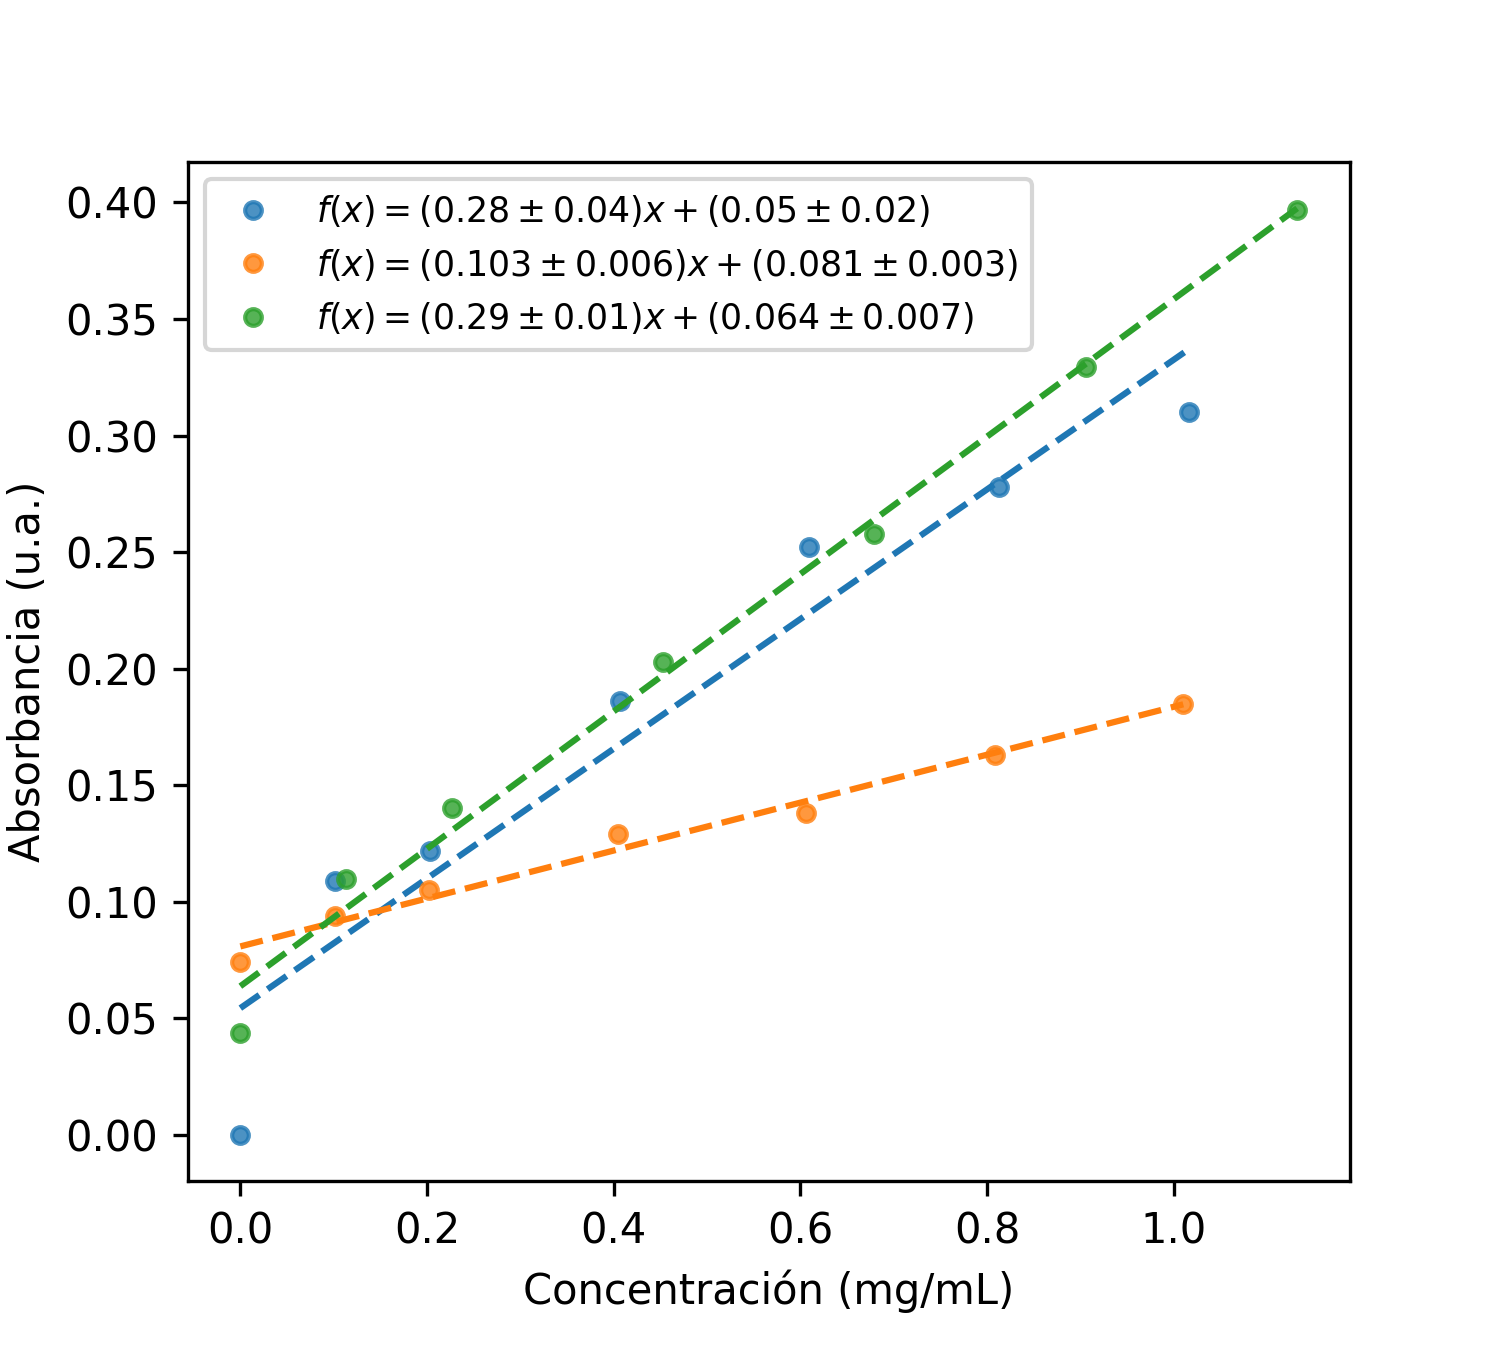
\includegraphics[width = 0.45\linewidth]{harinas_reg} & 
		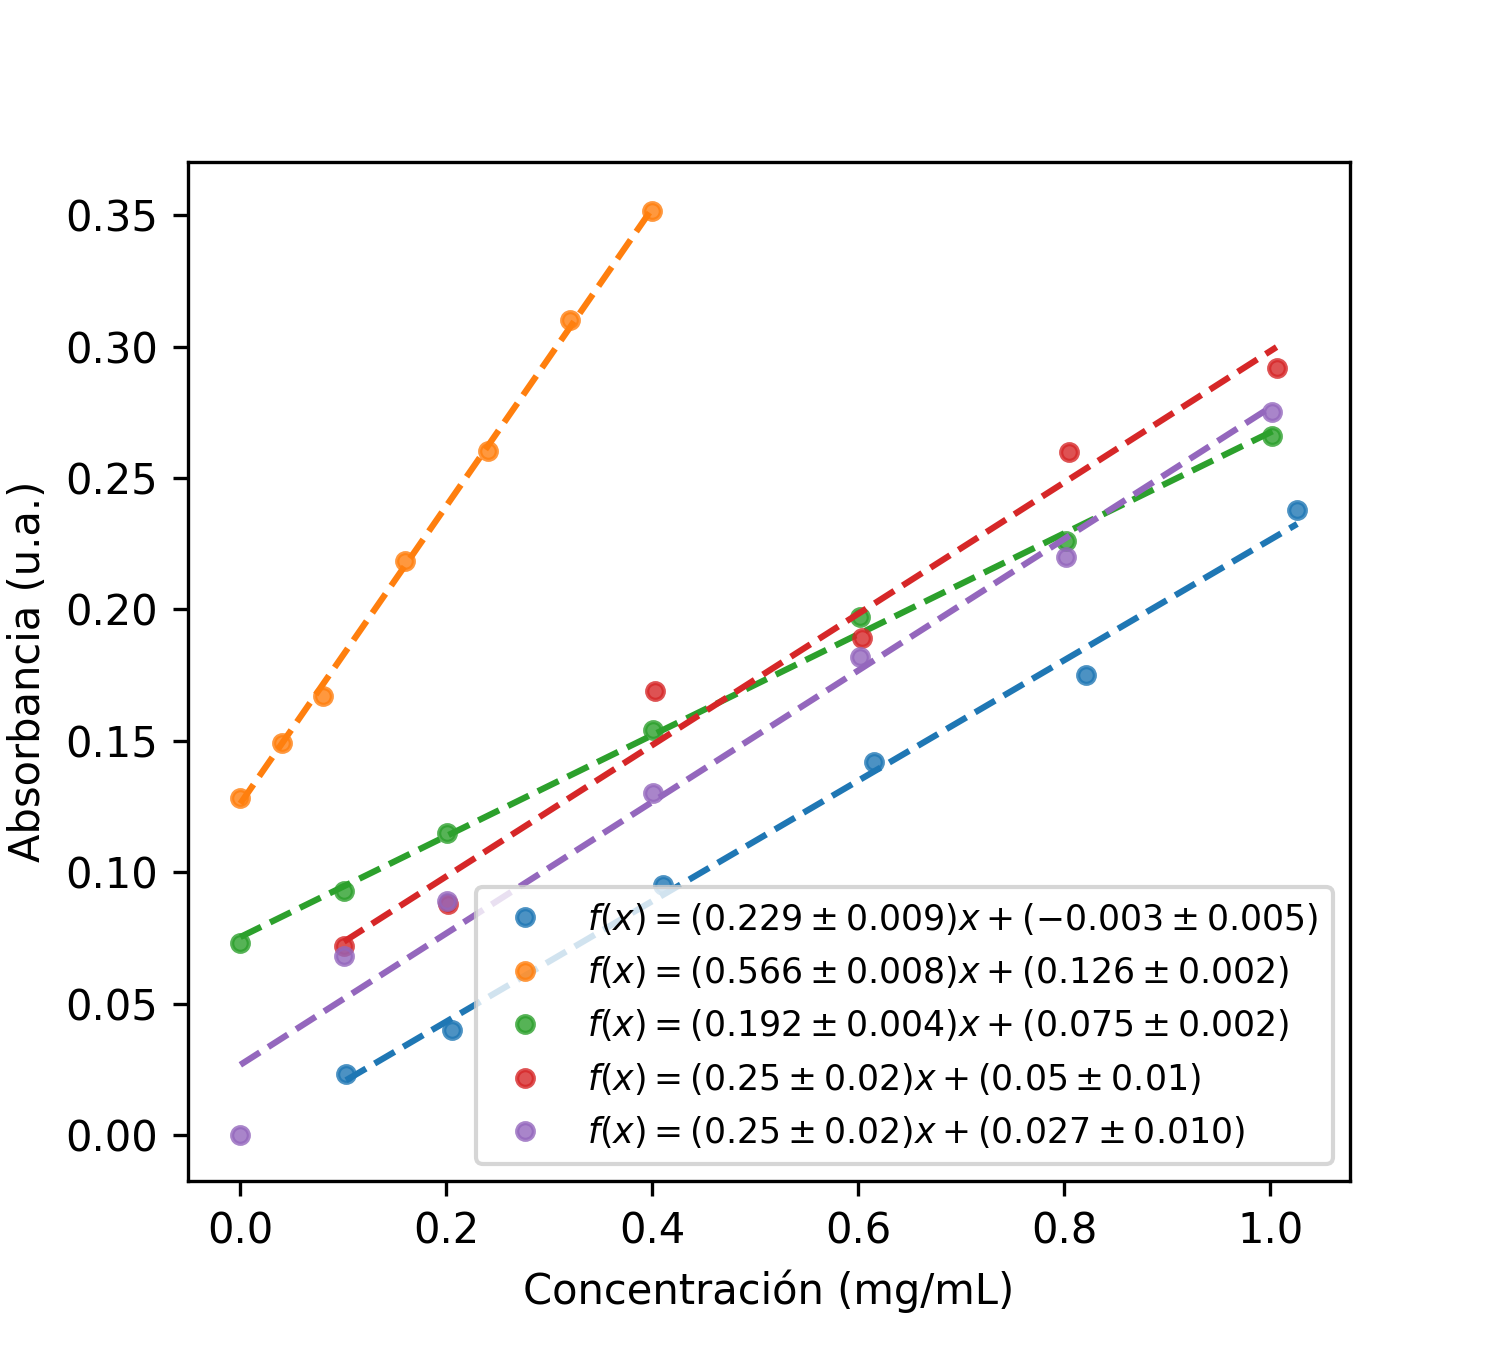
\includegraphics[width = 0.45\linewidth]{huevos_reg}
	\end{tabular}
	\caption{Curvas de calibraci\'on para la harina (izquierda) y huevo (derecha).}
	\label{fig: pendientes}
\end{figure*}
	
\section{Secci\'on experimental}
En un balon aforado de 250 mL fueron disueltos 0.38 g de sulfato de cobre (II) pentahidratado, y 1.5 g de tartrato de sofio y potasio tetrahidratado usando 75 mL de una soluci\'on de hidr\'oxido de sodio 10 \% preparada previamente. Posteriormente fue adicionado 0.25 g de yoduro de potasio y finalmente, la soluci\'on aforada. En un balón aparte fueron disueltos 1 g de cloruro de sodio en 100 mL de agua.
	\subsection{Preparaci\'on de la muestra}
		Cerca de 2 g de harina fueron disueltas en 10 mL de cloruro de sodio al 1 \%. La muestra disuelta fue centrifugada por 10 minuto a 2800 rpm. El sobrenadante fue aforado en 25 mL de de la soluci\'on de NaCl. En el caso de la clara de huevo, se realiz\'o una primera diluci\'on 1:10 usando cloruro de sodio al 10 \% en un bal\'on de 25 mL. Posteriormente se realizaron dos diluciones de 1 en 5, y 1 en 10, con NaCl en balones de 25 mL.
		
		\newpage
		
	\subsection{Preparaci\'on de las soluciones stock}
		Para el estudio de la prote\'ina en la harina, se prepar\'o una soluci\'on stock con concentraciones de 2.5 mg/mL de alb\'umica s\'erica y 2.5 mg/mL de globulina. Para la soluci\'on stock asociada con la alb\'umina de huevo, se pesaron 50 mg de ovoalb\'umina, los cuales fueron aforados en 10 mL de agua.

	\subsection{Curvas de calibraci\'on y medidas}
		Los patrones de las curvas de calibraci\'on fueron preparados realizando diluciones de 0.0, 0.2, 0.4, 0.8, 1.2, 1.6 y 2.0 mL de cada soluci\'on stock en 8 mL del reactivo de Biuret previamente preparado. De forma an\'aloga, se tomaron 2.0 mL de las soluciones de harina y huevo, las cuales se aforaron en balones de 10 mL usando el reactivo de Biuret. Todas las soluciones se dejaron reposar por cerca de 30 minutos, hasta observar que las muestras manten\'ian un color constante.
		
		Se construyeron las curvas de calibraci\'on a 571 nm usando celdas de pl\'astico y la soluci\'on de cloruro de sodio, previamente preparada, como blanco.
	
\section{Resultados y Discusi\'on}
	\begin{table}[h]
		\centering
		\caption{Cantidad de proteínas en las muestras de harina.}
		\label{tb: tabla1}
		\begin{tabular}{c|p{3cm}p{2.5cm}}
			\hline
			\textbf{Muestra} & \textbf{Concentración en solución (mg/mL)} & \textbf{Cantidad en 100 g de harina (g)}
			\\
			\hline
			Muestra 1 & 0.364 & 0.706 \\
			Muestra 2 & 0.227 & 0.284 \\
			Muestra 3 & 0.565 & 0.790 \\
			Muestra 4 & 0.273 & 0.324 \\
			\hline
		\end{tabular}
	\end{table}
	Como se describió en el procedimiento experimental se realizó una curva de calibración utilizando una solución stock de 5.08 mg/mL (2.57 mg/mL de albúmina y 2.51 mg/mL de globulina), haciendo una interpolación con la curva de calibración que se observa en la \autoref{fig: pendientes} se obtuvo los resultados que se muestran en la \autoref{tb: tabla1}, los datos obtenidos presentan un promedio de 0,526 g de proteínas por cada 100 g de harina con un desviación estándar de 0,259. Según lo reportado se debería esperar un total de 1,8 g de albúmina y globulina \cite{payne1979subunit}, sin embargo los resultados difieren ya que la extracción que se realizó no fue exhaustiva, asimismo los resultados presentan una alta deviación estándar ya que no se empleó la misma marca de harina entre los grupos.
%	
%	\begin{figure}[h]
%		\centering
%		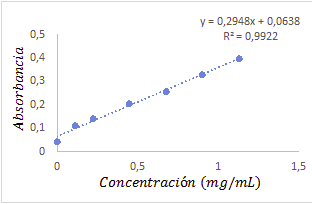
\includegraphics[width = \linewidth]{fig1}
%		\caption{Curva de calibración para la determinación de proteínas es harina de trigo.}
%		\label{fig: fig1}
%	\end{figure}

	En el caso de la alb\'umina de huevo, se realizaron dos diluciones a partir de una primera soluci\'on stock de 1:10 clara de huevo : NaCl (ac) 1 \%. La primera de estas corresponde con una disoluci\'on 1:10, y la segunda 1:5, las concentraciones calculadas a partir de las absorbancias reportadas por los distintos grupos de laboratorio, y sus curvas de calibraci\'on se muestran en la \autoref{tb: huevo_concentraciones}. Con el objetivo de determinar si los datos son suficientemente coherentes para la realizaci\'on de un an\'alisis estad\'istico entre grupos, para determinar el intervalo de confianza, se realiza la raz\'on entre la concentraci\'on obtenida para las disoluciones antes mencionadas, para la cual se deber\'ia obtener un factor de 2. Sin embargo, como se observa en la \autoref{tb: huevo_concentraciones}, no se evidencia ninguna relaci\'on constante para todos los 5 grupos, de hecho, los factores se pueden agrupar en 3 subgrupos: 1.15, $\approx$ 1.75 y $\approx$ 2.5. La presencia de 3 subgrupos en una muestra de 5, ocasiona que exista al menos 1 grupo con un \'unico dato, haciendo poco confiable un estudio estad\'istico, dada el taman\~o de la muestra.

	\begin{table}[h]
		\centering
		\caption{Concentraciones obtenidas para las dos diluciones de la soluci\'on stock medidas del huevo.}
		\label{tb: huevo_concentraciones}
		\begin{tabular}{c|cc|c}
			\hline
			\textbf{Grupo} & \textbf{1:10 (mg/mL)} & \textbf{1:5 (mg/mL)} & \textbf{Raz\'on} \\
			\hline
			1 & 1.7205 & 1.9869 & 1.15 \\
			2 & 0.0809 & 0.1979 & 2.45 \\
			3 & 0.2222 & 0.5711 & 2.57 \\
			4 & 0.7040 & 1.2596 & 1.79 \\
			5 & 0.3649 & 0.6327 & 1.73 \\
			\hline
		\end{tabular}
	\end{table}

	Para reportar el valor esperado de la prote\'ina del huevo con alg\'un intervalo de confianza, es necesario conocer a profundidad la distribuci\'on de los datos. En la \autoref{fig: dist} se muestra c\'omo se distribuyen las concentraciones inferidas para la ovoalb\'umina, mostrando que existe informaci\'on insuficiente para determinar la distribuci\'on real de la muestra, por otro lado el corrimiento horizontal para datos de un mismo color (grupo), resalta el argumento anterior de una falta de coherencia en la informaci\'on reportada. Esto \'ultimo es de particular importancia dado que se puede argumentar que dos huevos extra\'idos de ambientes completamente distintos han de tener una concentraci\'on de prote\'ina diferente, si bien los autores consideran este argumento como v\'alido, para un mismo grupo \'este carece de aplicaci\'on, por lo cual, la disperci\'on en la concentraci\'on obtenida deber\'ia ser considerablemente menor.
	\begin{figure}[h]
		\centering
		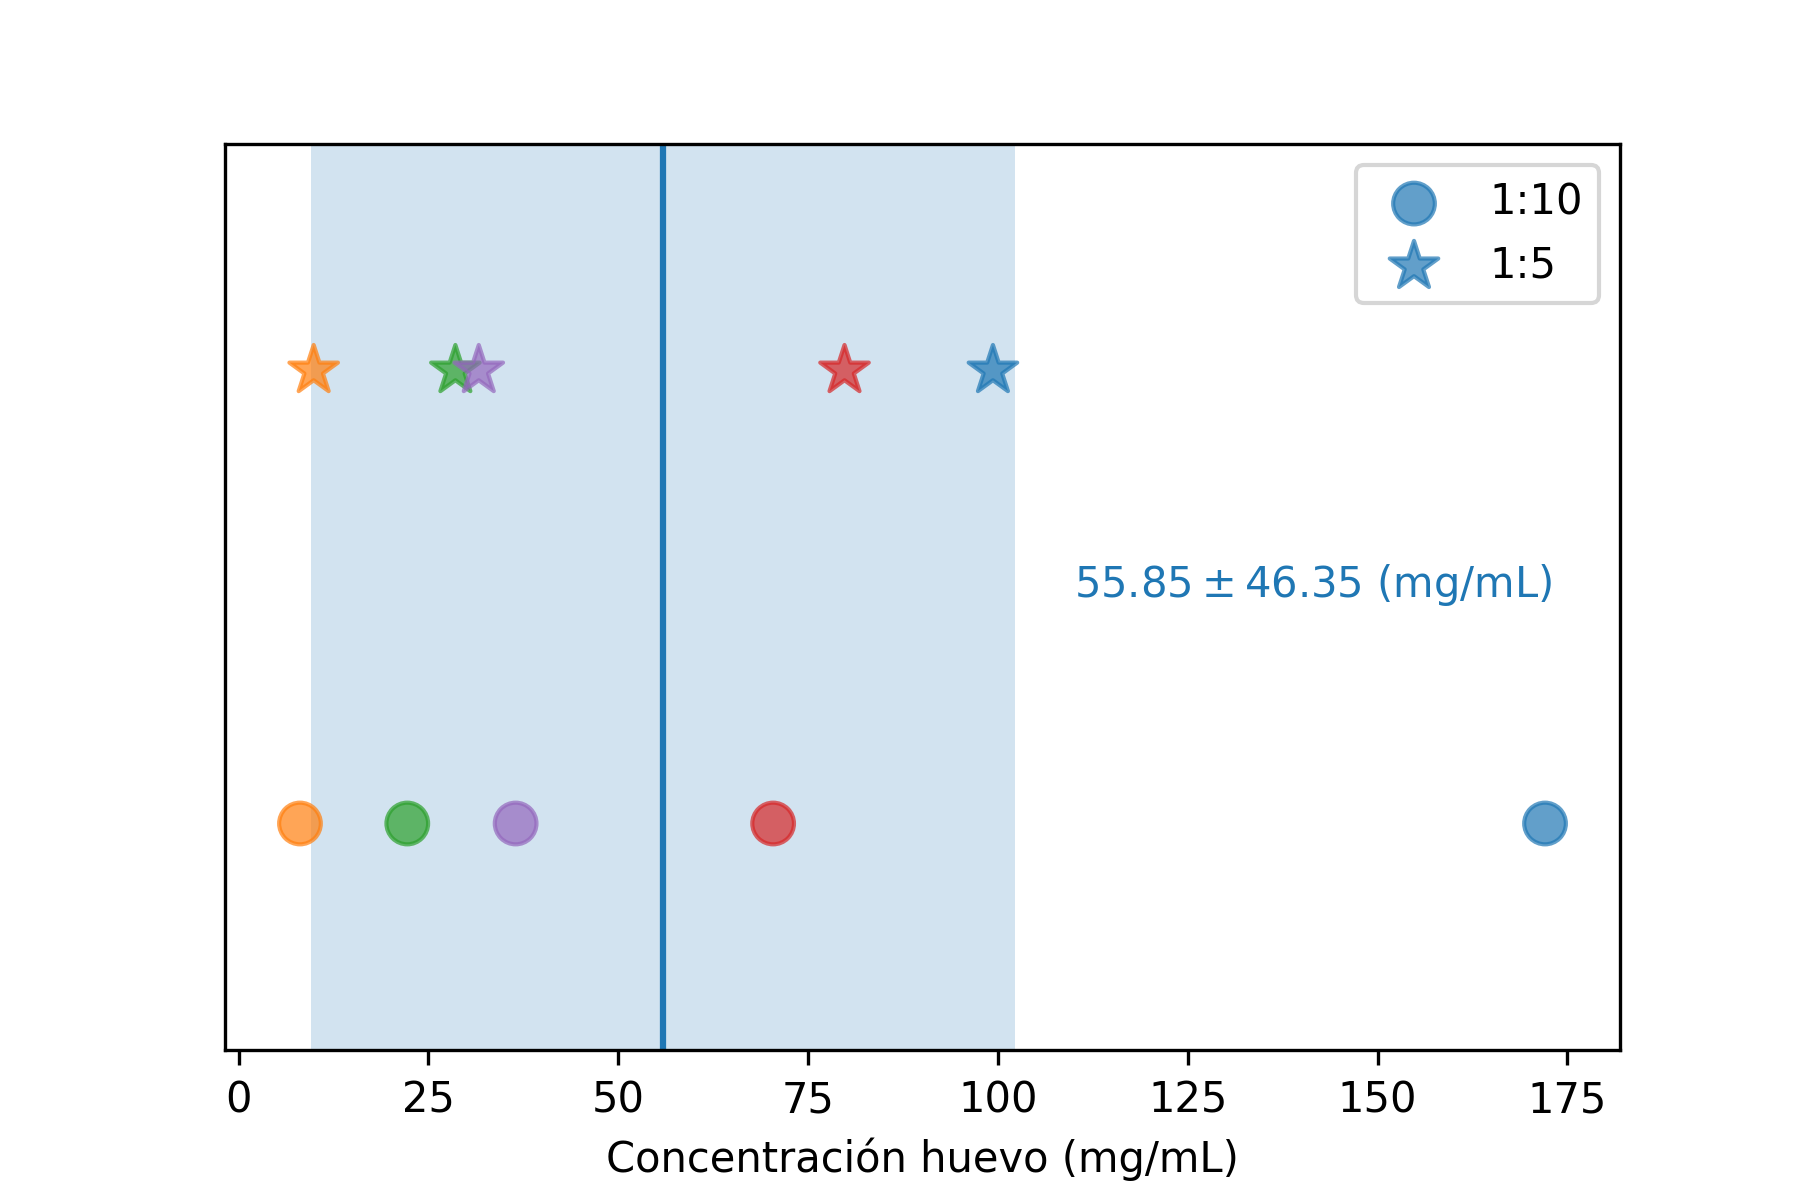
\includegraphics[width=\linewidth]{concentraciones}
		\caption{Distribuci\'on de la concentraci\'on prote\'inas en la clara de huevo a partir de los datos. Usando c\'irculos se muestran las concentraciones inferidas a partir de las disoluciones 1:10, cada color se encuentra asociado a las pendientes de la \autoref{fig: pendientes}. La l\'inea azul muestra el promedio de los datos, y el \'area coloreada la regi\'on entre $\mu \pm \sigma$.}
		\label{fig: dist}
	\end{figure}

	A pesar de las incongruencias antes mencionadas, se reporta la concentraci\'on de ovoalb\'umina en la clara de huevo en $(6\pm5)\times10^{1}$ mg/mL. Dos posibles explicaciones a los resultados son propuestas, por un lado, la preparaci\'on de la muestra del huevo es considerablemente m\'as compleja que para la harina, esta complejidad puede explicar los disperci\'on de los resultados entre grupos. En el caso de los valores obtenidos para un mismo grupo, existe la posibilidad que la reacci\'on de las prote\'inas con el reactivo de Biuret no haya llego a su fin, y lo que se observa sea un efecto cin\'etico, en la que unas muestras hayan progresado m\'as en la reacci\'on que otras. 
	
	\newpage

\section{Conclusiones}
	Se realizó la extracción de proteínas como albúmina, globulina y ovoalbúmina de matrices de harina de trigo y clara de huevo. Empleando estándares de estas proteínas se realizó una curva de calibración y haciendo uso de esta y mediante interpolación lineal, se determinó la cantidad de proteínas presentes en las matrices. Se puede observar que mediante el empleo del reactivo de Biuret se puede llevar a cabo cuantificaciones de forma sencilla, dando lugar a cantidades de proteína en 100 g de harina entre 0.706 g y 0.284 g, para el caso de la ovoalbúmina, se cuantificó la cantidad protéica entre 10 mg/mL y 110 mg/mL.
	
	
%----------------------------------------------------------------------------------------
%	REFERENCE LIST
%----------------------------------------------------------------------------------------
\phantomsection
\bibliography{informe}
\bibliographystyle{unsrt}

%----------------------------------------------------------------------------------------
%\newpage
%\onecolumn
%\section{Informaci\'on suplementaria}\label{sec: complementaria}
\end{document}